{\textbf{1.超标量技术}}

超标量技术的每个时钟周期不像以前的普通指令流水线只能执行一条指令的某个阶段,而是\textbf{可以并发执行多条独立指令},为此就需要配置多个功能部件,如下图所示。

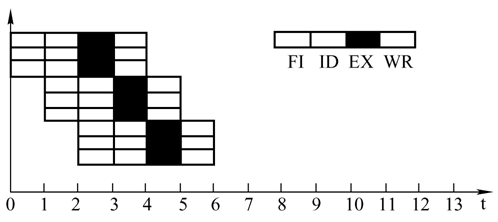
\includegraphics[width=3.33333in,height=1.48958in]{png-jpeg-pics/70CCDEFF7D2922032E9EC5783A4F7AF9.png}

{\textbf{2.超级流水线}}

典型的流水线是将每一条机器指令分成5步,即取指、译码、取操作数、执行和回写。在理想条件下,平均每个时钟周期可以完成一条指令。而所谓的超级流水线是\textbf{将机器指令划分为更多级的操作},以减轻每一级的复杂程度。在流水线的每一步中,如果需要执行的逻辑操作少一些,那么每一步就可以在较短的时间内完成,如下图所示。

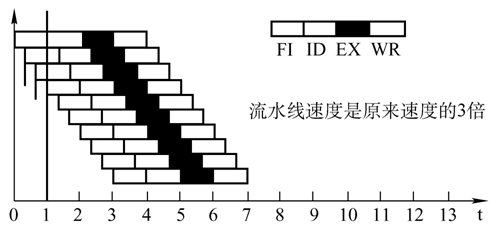
\includegraphics[width=3.33333in,height=1.54167in]{png-jpeg-pics/0E0DE9C31F4E78B16AF9BAA8C5D4D0D3.png}

{\textbf{3.超长指令字}}

由编译程序挖掘出指令潜在的并行性,\textbf{将多条能并行操作的指令组合成一条具有多个操作码字段的超长指令字}(可达几百位),为此需要采用多个处理部件,如下图所示。\\
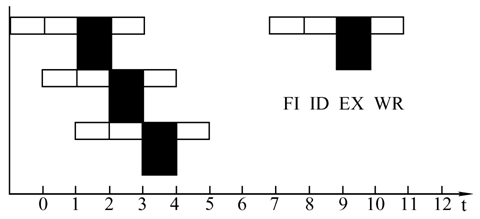
\includegraphics[width=3.33333in,height=1.52083in]{png-jpeg-pics/387B07E477E1BD300EECA9B68FAB749D.png}

{\textbf{4.动态流水线}}

动态流水线就是\textbf{多种运算可以同时进行},而静态流水线只能是一种运算进行完再进行下一种运算。
